
%----------------------------------------------------------------------------------------
%	PACKAGES AND THEMES
%----------------------------------------------------------------------------------------

\documentclass{beamer}
\usepackage[utf8]{inputenc}
\usetheme{Berkeley}
\usecolortheme{dove}

\usepackage{graphicx} % Allows including images
\usepackage{booktabs} % Allows the use of \toprule, \midrule and \bottomrule in tables
\newcommand{\dd}{\; \mathrm{d}}
\usepackage{amsmath}
%----------------------------------------------------------------------------------------
%	TITLE PAGE
%----------------------------------------------------------------------------------------

\title[Years Lost]{Life lost, lifesaving, and causes of death.}
\author[Riffe \& Sol\'{e}]
{
Tim Riffe \inst{1} \and A{\"i}da Sol\'{e} Aur\'{o} \inst{2}}
\institute % (optional)
{
  \inst{1}%
  Department of Demography, \\
  University of California, Berkeley \\
  %\raggedleft{
  %
\includegraphics[width=1.2cm]{Figures/demogcrest}
  %
\includegraphics[width=1.2cm]{Figures/ucbseal1}}\\
  \and
  \inst{2} Universitat Pompeu Fabra
  %\raggedleft{
\includegraphics[height=1cm]{Figures/UPFcmyk}} }
%\titlegraphic{
\includegraphics[width=1.5cm]{Figures/demogcrest}~~
%   
\includegraphics[width=1.5cm]{Figures/ucbseal1}~~
%   
\includegraphics[height=1.5cm]{Figures/UPFcmyk}
}
%\date[May 2, 2015] % (optional)
%{PAA annual meeting\\ Session 234}
\begin{document}
% remove figure headers
\setbeamertemplate{caption}{\raggedright\insertcaption\par}

% ------------------------------------------
% title page for now. see about logos
%\begin{frame}
%\titlepage % Print the title page as the first slide
%\end{frame}
\begin{frame}[plain]

\vspace{3em}
\LARGE Life lost, lifesaving, and causes of death\\
----- Ghost demography -----
\\
\vspace{3 mm}
\normalsize Tim Riffe$^1$ \& A{\"i}da Sol\'{e} Aur\'{o}$^2$\\
\vspace{3 mm}
 $^1$ Department of Demography, \\
  \hspace{2mm} University of California, Berkeley \\
  $^2$ Universitat Pompeu Fabra\\
  \vspace{5 mm}
  PAA 2015 Annual Meeting \\
  Session 234, Saturday, May 2\\
  \vspace{5 mm}
  
\includegraphics[width=1.5cm]{Figures/demogcrest}\hspace{.5cm}
  
\includegraphics[width=1.5cm]{Figures/ucbseal1}\hspace{3cm}
  
\includegraphics[height=1.2cm]{Figures/UPFcmyk}
\end{frame}


% good way to start. we have trends and levels in rates and expectancies,
% survival, etc
\begin{frame}
\frametitle{Mortality measurement}
\begin{description}
\item[\textbf{lifetable}:] purged of structure
\item[\textbf{counts}:] structure $\times$ intensity
\item[\textbf{combo}:] Person Years of Life Lost (PYLL),
\underline{\hspace{1cm}},
\ldots
\end{description}

\end{frame}

\section{All-cause}
\begin{frame}
\frametitle{PYLL}
Person years of life lost
\begin{align}
\text{PYLL} &= \int_0^\omega D(a) \cdot e(a) \dd a \\
\text{PYLL}^c &= \int_0^\omega D^c(a) \cdot e(a) \dd a
\end{align}
%(mention that there are decreasing returns to $\mu(a)$ improvements, since
%$D(a)$ decreases, but $e(a)$ increases = ambiguous change in PYLL?)
\end{frame}


\begin{frame}
\frametitle{PYLL \& friends}
\vspace{-1cm}
\begin{figure}[b]
    \centering
    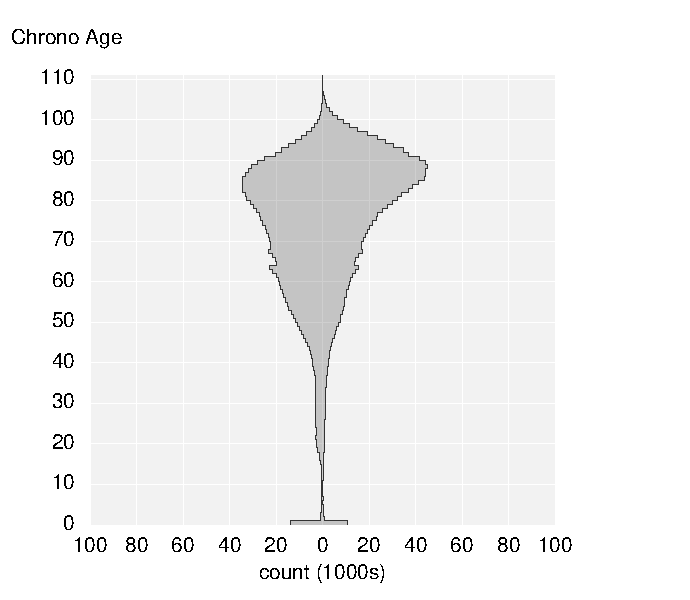
\includegraphics[scale=.7]{Figures/f1_Da.pdf}
    \caption{$D(a)$ (USA, 2010)}
\end{figure} 
\end{frame}
%%%%%%%%%%%%%%%%%%%%%%%%%%%%%%%%%%%%%%%%%%%%%%%%%%
%% D(y) --- lifespans foregone                  %%
%%%%%%%%%%%%%%%%%%%%%%%%%%%%%%%%%%%%%%%%%%%%%%%%%%
%\begin{frame}
%\frametitle{PYLL \& friends}
%\vspace{-1cm}
%\begin{figure}[b]
%    \centering
%    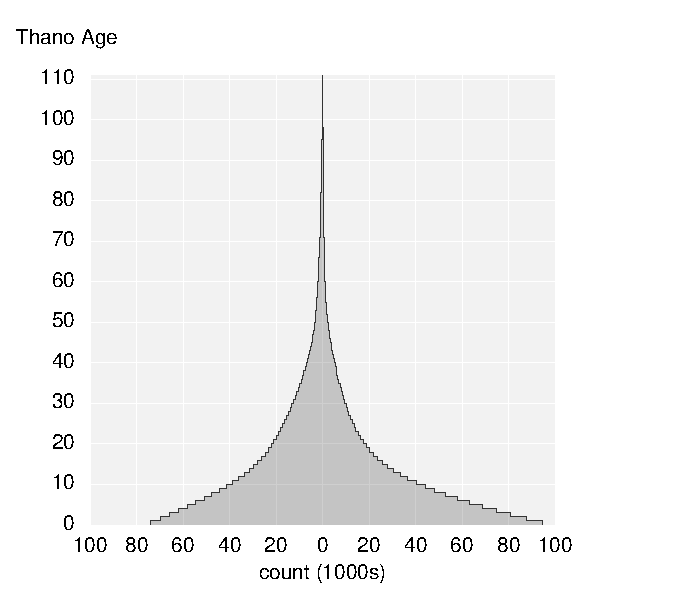
\includegraphics[scale=.7]{Figures/f2_Dy.pdf}
%    \caption{$D(y)$ (USA, 2010)}
%\end{figure} 
%\end{frame}
%%%%%%%%%%%%%%%%%%%%%%%%%%%%%%%%%%%%%%%%%%%%%%%%%%
%% D(a) --- lifespans foregone                  %%
%%%%%%%%%%%%%%%%%%%%%%%%%%%%%%%%%%%%%%%%%%%%%%%%%%
\begin{frame}
\frametitle{PYLL \& friends}
\vspace{-1cm}
\begin{figure}[b]
    \centering
    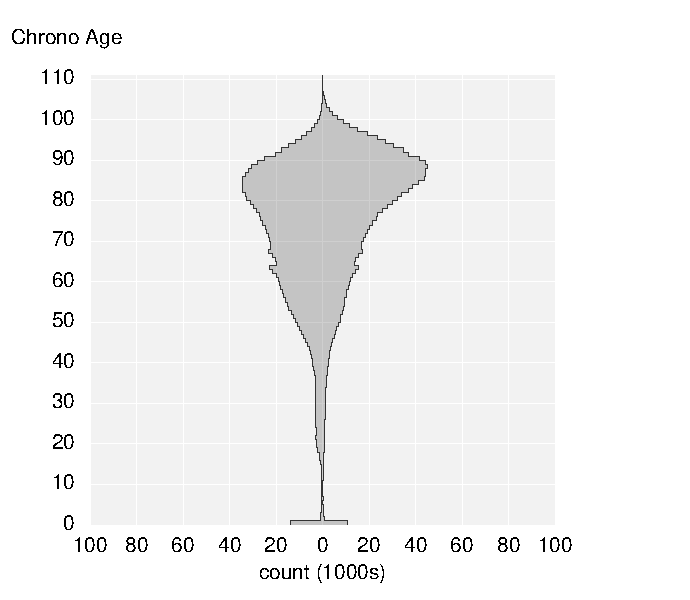
\includegraphics[scale=.7]{Figures/f3_Da.pdf}
    \caption{$D(a)$ (USA, 2010)}
\end{figure} 
\end{frame}
%%%%%%%%%%%%%%%%%%%%%%%%%%%%%%%%%%%%%%%%%%%%%%%%%%
%% D(a) - lifespans foregone                    %%
%%%%%%%%%%%%%%%%%%%%%%%%%%%%%%%%%%%%%%%%%%%%%%%%%%
%\begin{frame}
%\frametitle{PYLL \& friends}
%\vspace{-1cm}
%\begin{figure}[b]
%    \centering
%    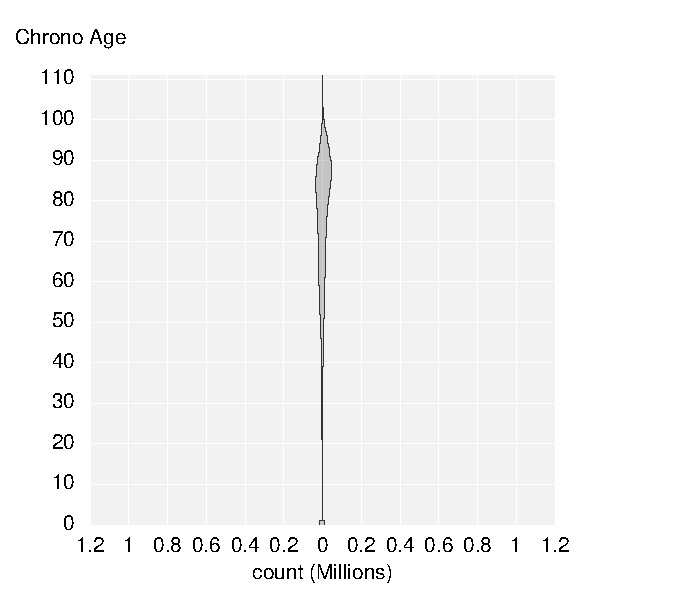
\includegraphics[scale=.7]{Figures/f4_Da.pdf}
%    \caption{$D(a)$ (USA, 2010)- changed scale}
%\end{figure} 
%\end{frame}
%%%%%%%%%%%%%%%%%%%%%%%%%%%%%%%%%%%%%%%%%%%%%%%%%%
%% D(a)e(a) - PYLL(a)                           %%
%%%%%%%%%%%%%%%%%%%%%%%%%%%%%%%%%%%%%%%%%%%%%%%%%%
\begin{frame}
\frametitle{PYLL \& friends}
\vspace{-1cm}
\begin{figure}[b]
    \centering
    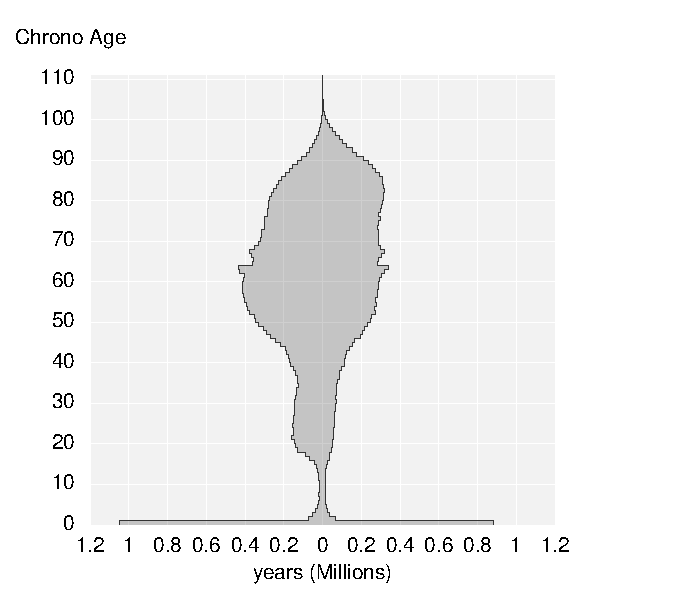
\includegraphics[scale=.7]{Figures/f5_Daea.pdf}
    \caption{$PYLL(a)$ (USA, 2010)}
\end{figure} 
\end{frame}
%%%%%%%%%%%%%%%%%%%%%%%%%%%%%%%%%%%%%%%%%%%%%%%%%%
%% Ages won                                     %%
%%%%%%%%%%%%%%%%%%%%%%%%%%%%%%%%%%%%%%%%%%%%%%%%%%
\begin{frame}
\frametitle{PYLL \& friends}
\vspace{-1cm}
\begin{figure}[b]
    \centering
    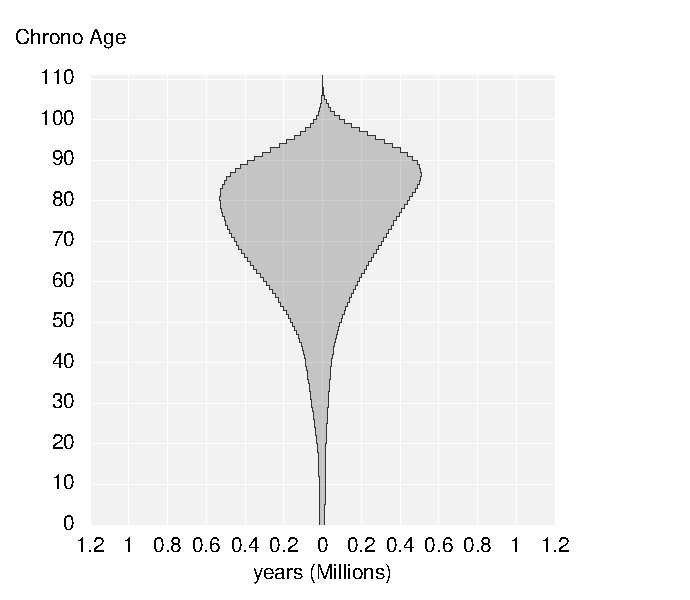
\includegraphics[scale=.7]{Figures/f6_AgesWon.pdf}
    \caption{$G(a)$ (USA, 2010)}
\end{figure} 
\end{frame}

%%%%%%%%%%%%%%%%%%%%%%%%%%%%%%%%%%%%%%%%%%%%%%%%%%%%%%%%%%%%%%%
%  I'm leaning toward just showing this last plot for causes %%
%%%%%%%%%%%%%%%%%%%%%%%%%%%%%%%%%%%%%%%%%%%%%%%%%%%%%%%%%%%%%%%
\section{Causes}
\begin{frame}
\frametitle{PYLL \& friends, causes of death}
\vspace{-1cm}
\begin{figure}[b]
    \centering
    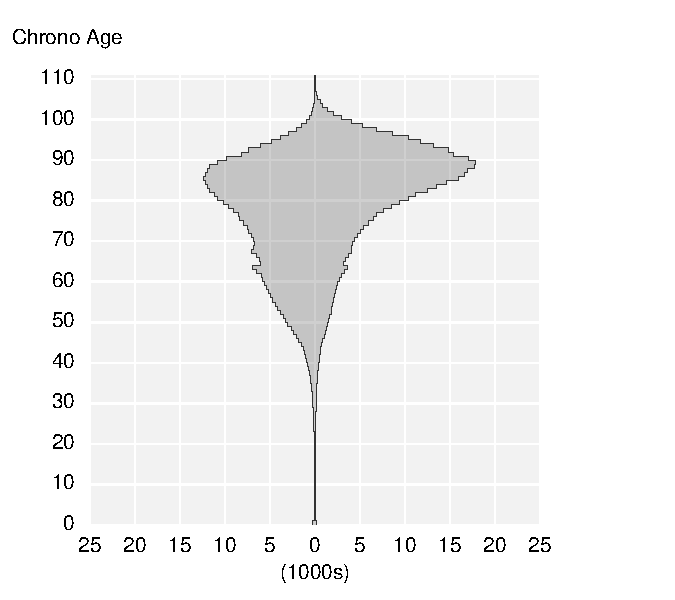
\includegraphics[scale=.7]{Figures/f7_Dac.pdf}
    \caption{$D(a)$ Cardio (USA, 2010)}
\end{figure} 
\end{frame}

\begin{frame}
\frametitle{PYLL \& friends}
\vspace{-1cm}
\begin{figure}[b]
    \centering
    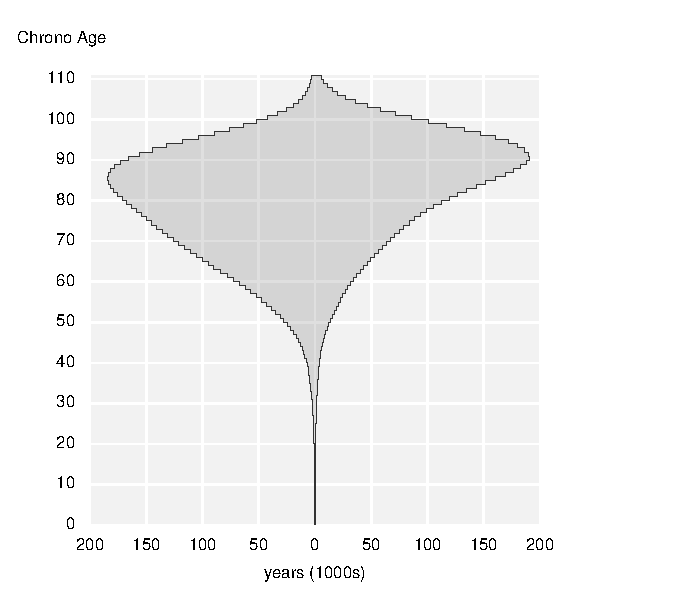
\includegraphics[scale=.7]{Figures/f8_AgesWonc.pdf}
    \caption{$G(a)$ Cardio (USA, 2010)}
\end{figure} 
\end{frame}

\section{Comparisons}

\begin{frame}
\frametitle{PYLL \& friends, decompose}
\vspace{-1cm}
\begin{figure}[b]
    \centering
    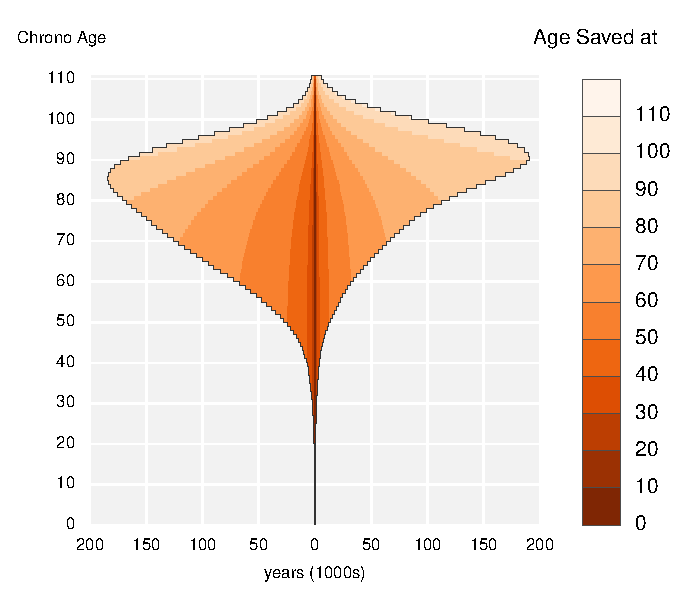
\includegraphics[scale=.7]{Figures/f9_AgesWoncdec.pdf}
    \caption{$G(a+y|a)$ Cardio (USA, 2010)}
\end{figure} 
\end{frame}

\begin{frame}
\frametitle{PYLL \& friends, compare causes}
\vspace{-1cm}
\begin{figure}[b]
    \centering
    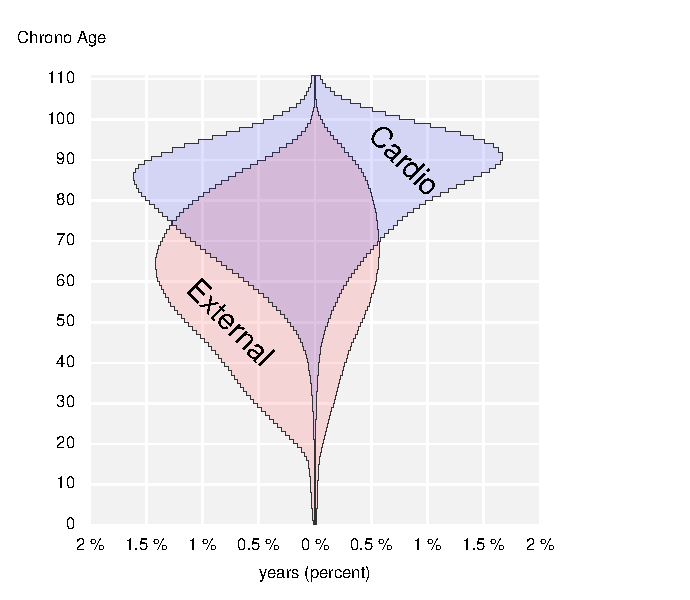
\includegraphics[scale=.7]{Figures/f11_AgesWoncomp.pdf}
    \caption{$G(a)$ Cardio vs External (USA, 2010)}
\end{figure} 
\end{frame}

\begin{frame}
\frametitle{PYLL \& friends, compare populations}
\vspace{-1cm}
\begin{figure}[b]
    \centering
    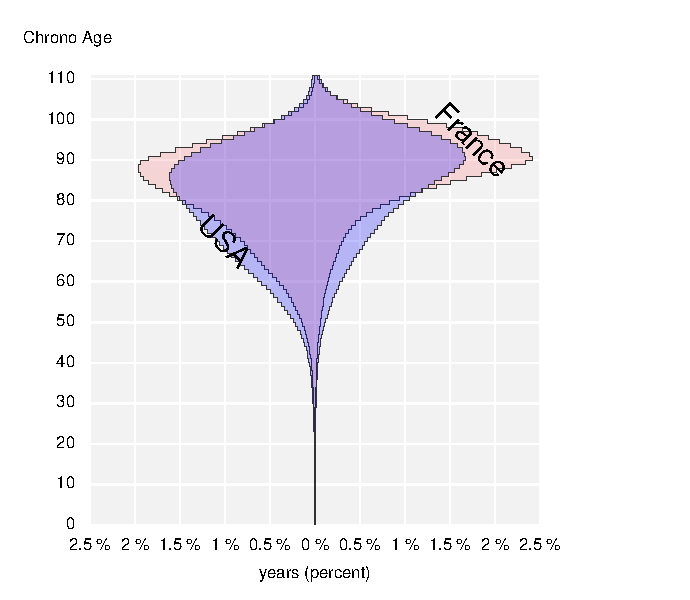
\includegraphics[scale=.7]{Figures/f12_AgesWoncountries.pdf}
    \caption{$G(a)$ Cardio (USA vs France, 2010)}
\end{figure} 
\end{frame}

\begin{frame}
\frametitle{PYLL \& friends, compare with stationary}
\vspace{-1cm}
\begin{figure}[b]
    \centering
    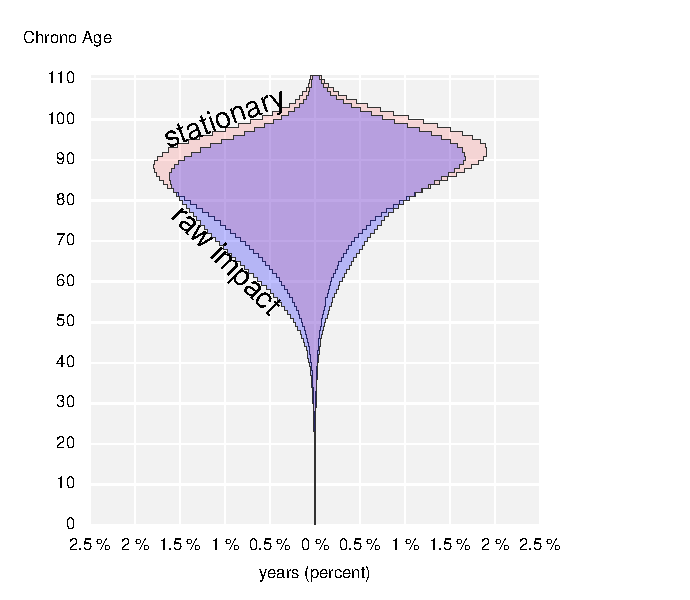
\includegraphics[scale=.7]{Figures/f13_AgesWonstationary.pdf}
    \caption{$G(a)$ Cardio (Raw impact versus stationary, USA, 2010)}
\end{figure} 
\end{frame}

\begin{frame}
\frametitle{PYLL \& friends, summaries}
\begin{description}
\item[$\bar{A}$] mean chrono age of $G$
\item[$\bar{Y}$] mean thanatological age of $G$
\end{description}
\end{frame}

\section{Rates}
\begin{frame}
\frametitle{PYLL \& friends, rates}
\begin{equation}
\mu^G(a) = \frac{G(a)}{P^F(a)}
\end{equation}
The lives that \textbf{would} have passed through age $a$ divided by the lives
that \textbf{will} pass through $G(a)$.
\end{frame}

\begin{frame}
\frametitle{PYLL \& friends, rates}
\vspace{-1cm}
\begin{figure}[b]
    \centering
    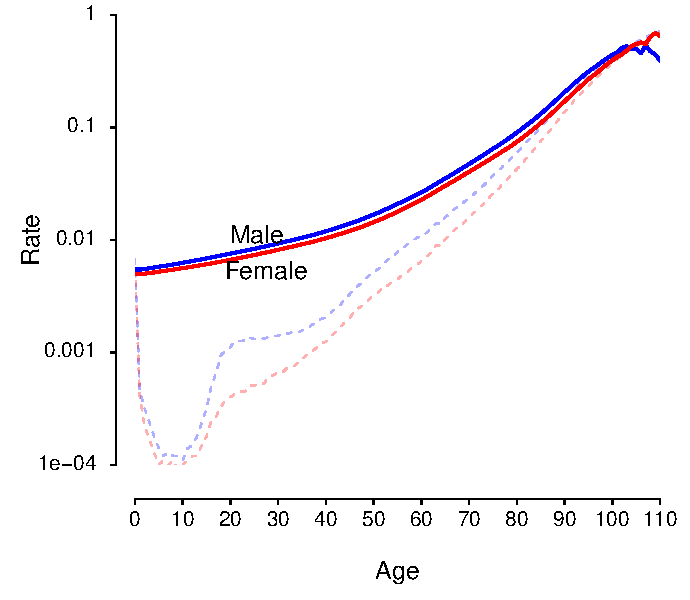
\includegraphics[scale=.7]{Figures/f14_linerate.pdf}
    \caption{$G(a)$ (male and female, USA, 2010)}
\end{figure} 
\end{frame}

\section{Conclusions}
\begin{frame}
\frametitle{PYLL \& friends, new material}

Counts, years, rates, impacts

\end{frame}



\begin{frame}[plain]

\vspace{3em}
\LARGE Life lost, lifesaving, and causes of death\\
\vspace{3 mm}
\normalsize Tim Riffe$^1$ \& A{\"i}da Sol\'{e} Aur\'{o}$^2$\\
\vspace{10 mm}
Thank you!\\
\vspace{3mm}
tim.riffe@gmail.com\\
Aida's email here \\ 
  \vspace{15 mm}
  
\includegraphics[width=1.5cm]{Figures/demogcrest}\hspace{.5cm}
  
\includegraphics[width=1.5cm]{Figures/ucbseal1}\hspace{3cm}
  
\includegraphics[height=1.2cm]{Figures/UPFcmyk}
\end{frame}

\end{document}







